\documentclass[11pt]{article}
\usepackage{geometry}
\geometry{a4paper, left=20mm, top=20mm}
\usepackage{amsmath}
\usepackage{graphicx}
\usepackage{hyperref}
\usepackage[T1]{fontenc}
\usepackage{polski}
\usepackage[utf8]{inputenc}

\usepackage{xcolor}

\usepackage{listings}
\usepackage{xcolor}

\definecolor{codegreen}{rgb}{0,0.6,0}
\definecolor{codegray}{rgb}{0.5,0.5,0.5}
\definecolor{codepurple}{rgb}{0.58,0,0.82}
\definecolor{backcolour}{rgb}{1,1,1}

\lstdefinestyle{mystyle}{
    backgroundcolor=\color{backcolour},   
    commentstyle=\color{codegreen},
    keywordstyle=\color{magenta},
    numberstyle=\tiny\color{codegray},
    stringstyle=\color{codepurple},
    basicstyle=\ttfamily\footnotesize,
    breakatwhitespace=false,         
    breaklines=true,                 
    captionpos=b,                    
    keepspaces=true,                 
    numbers=left,                    
    numbersep=5pt,                  
    showspaces=false,                
    showstringspaces=false,
    showtabs=false,                  
    tabsize=2
}

\lstset{style=mystyle}

\title{Aplikacja książka kucharska}
\author{Mikołaj Kubik}

\begin{document}
\maketitle
\section{Wstęp}
Celem projektu było stworzenie aplikacji webowej, będącej publiczną książką kucharską. Użytkownicy mogą dodawać nowe składniki
oraz tworzyć z nich przepisy a także dodawać komentarze do istniejących przepisów. W bazie danych przechowywane są wartości 
odżywcze poszczególnych składników, dzięki czemu użytkownik może lepiej dopasować dany przepis do swoich preferencji żywieniowych.

\section{Architektura techniczna}
\subsection{Wykorzystane narzędzia}
\begin{itemize}
    \item Docker -  utworzenie zamkniętego ekosystemu zawierającego bazę danych, API oraz aplikację frontendową. Docker compose budujący infrastrukturę aplikacji korzystając z obrazu bazy danych SQL server oraz zdefiniowanych na potrzebę projektu plików Dockerfile dla frontendu i backendu,
    \item Django 
    \begin{itemize}
        \item obługa bazy danych Django ORM
        \item Django Rest Framework - obsługa interfejsu API
        \item pyodbc, django-mssql-backend - podłączenie bazy danych mssql do aplikacji django
    \end{itemize}
    \item React - obsługa interfejsu użytkownika - obustronnej komunikacji z serwerem
    \item MS SQL - baza danych
\end{itemize}
\subsection{Baza danych}
\subsubsection{Diagram bazy danych}
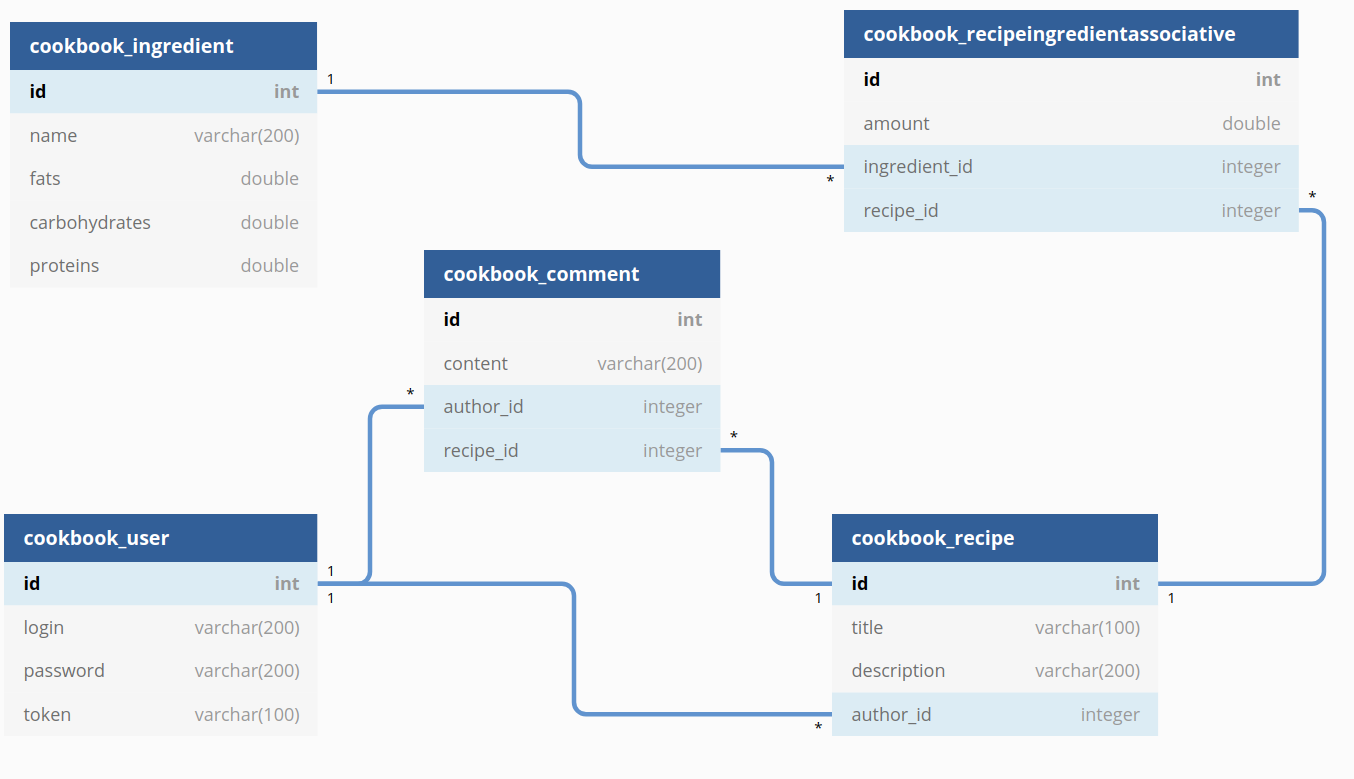
\includegraphics[width=15.5cm]{db_diagram.png}
\subsubsection{Skrypt tworzący bazę danych}
\lstinputlisting[language=SQL]{script.sql}
\subsection{Opis tabel}
Baza danych składa się z czterech głównych tabel oraz tabeli obsługującej relację
wiele do wielu pomiędzy przepisami i składnikami.
\begin{itemize}
    \item Cookbook\_recipe: tabela zawierająca przepisy
    \begin{itemize}
        \item id
        \item title: nazwa przepisu
        \item description: opis przepisu
        \item author\_id: id autora przepisu
    \end{itemize}
    \item Cookbook\_ingredient: tabela reprezentująca składnik
    \begin{itemize}
        \item id
        \item name: nazwa składnika
        \item fats: zawartość tłuszczy w 100g składnika
        \item carbohydrates: zawartość węglowodanów w 100g składnika
        \item proteins: zawartość białka w 100g składnika
        \item calories: ilość kalorii w 100g składnika
    \end{itemize}
    \item Cookbook\_recipeingredientassociative: tabela łącząca wiele do wielu składniki i przepisy
    \begin{itemize}
        \item id
        \item amount: ilość składnika w przepisie w gramach
        \item ingredient\_id: id składnika
        \item recipe\_id: id przepisu
    \end{itemize}
    \item User: tabela zawierająca dane użytkownika
    \begin{itemize}
        \item id
        \item login: login
        \item password: hasło
        \item token: token, któremu musi odpowiadać cookie w żądaniach dodawania nowych przepisów i komentarzy
    \end{itemize}
    \item Cookbook\_comment: tabela zawierająca komentarze do przepisów
    \begin{itemize}
        \item id
        \item content: treść komentarza
        \item author\_id: id autora komentarza
        \item recipe\_id: id komentowanego przepisu
    \end{itemize}
\end{itemize}


\section{Strona serwerowa}
\subsection{Definicja bazy danych w pythonie}
\lstinputlisting[language=Python]{../backend/CookBookApp/CookBook/models.py}
\subsection{Serializery}
Dane w większości przechodziły jedynie podstawową walidację - dotyczącą jedynie 
zadeklarowanego typu jednak w przypadkach tworzenia nowego przepisu lub dodawania komentarza
w miejsce autora wstawiany był obecnie uwierzytelniony użytkownik.
\lstinputlisting[language=Python]{../backend/CookBookApp/CookBook/serializers.py}

\section{Dokumentacja aplikacji}
\subsection{Dodawanie składników}
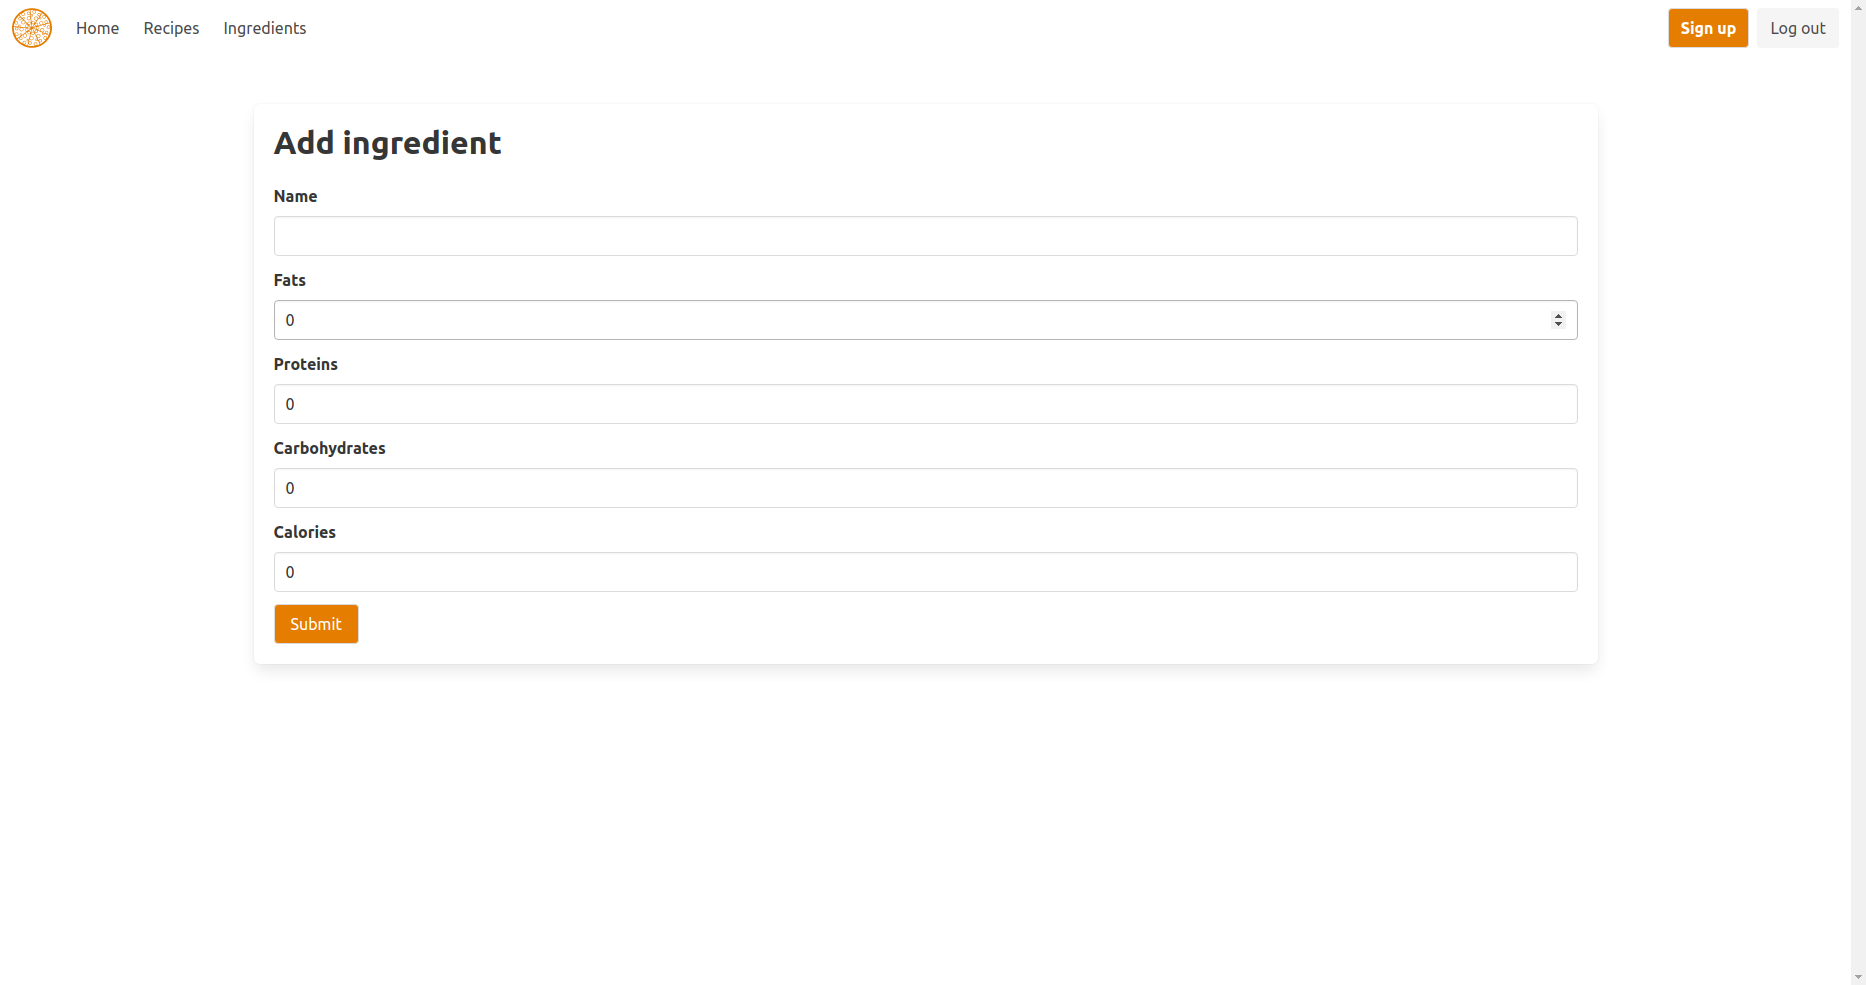
\includegraphics[width=15.5cm]{add_ingredient.png}
\newline
Uwierzytelniony użytkownik może dodać nowy składnik i jego wartości odżywcze
\subsection{Wyświetlanie listy składników}
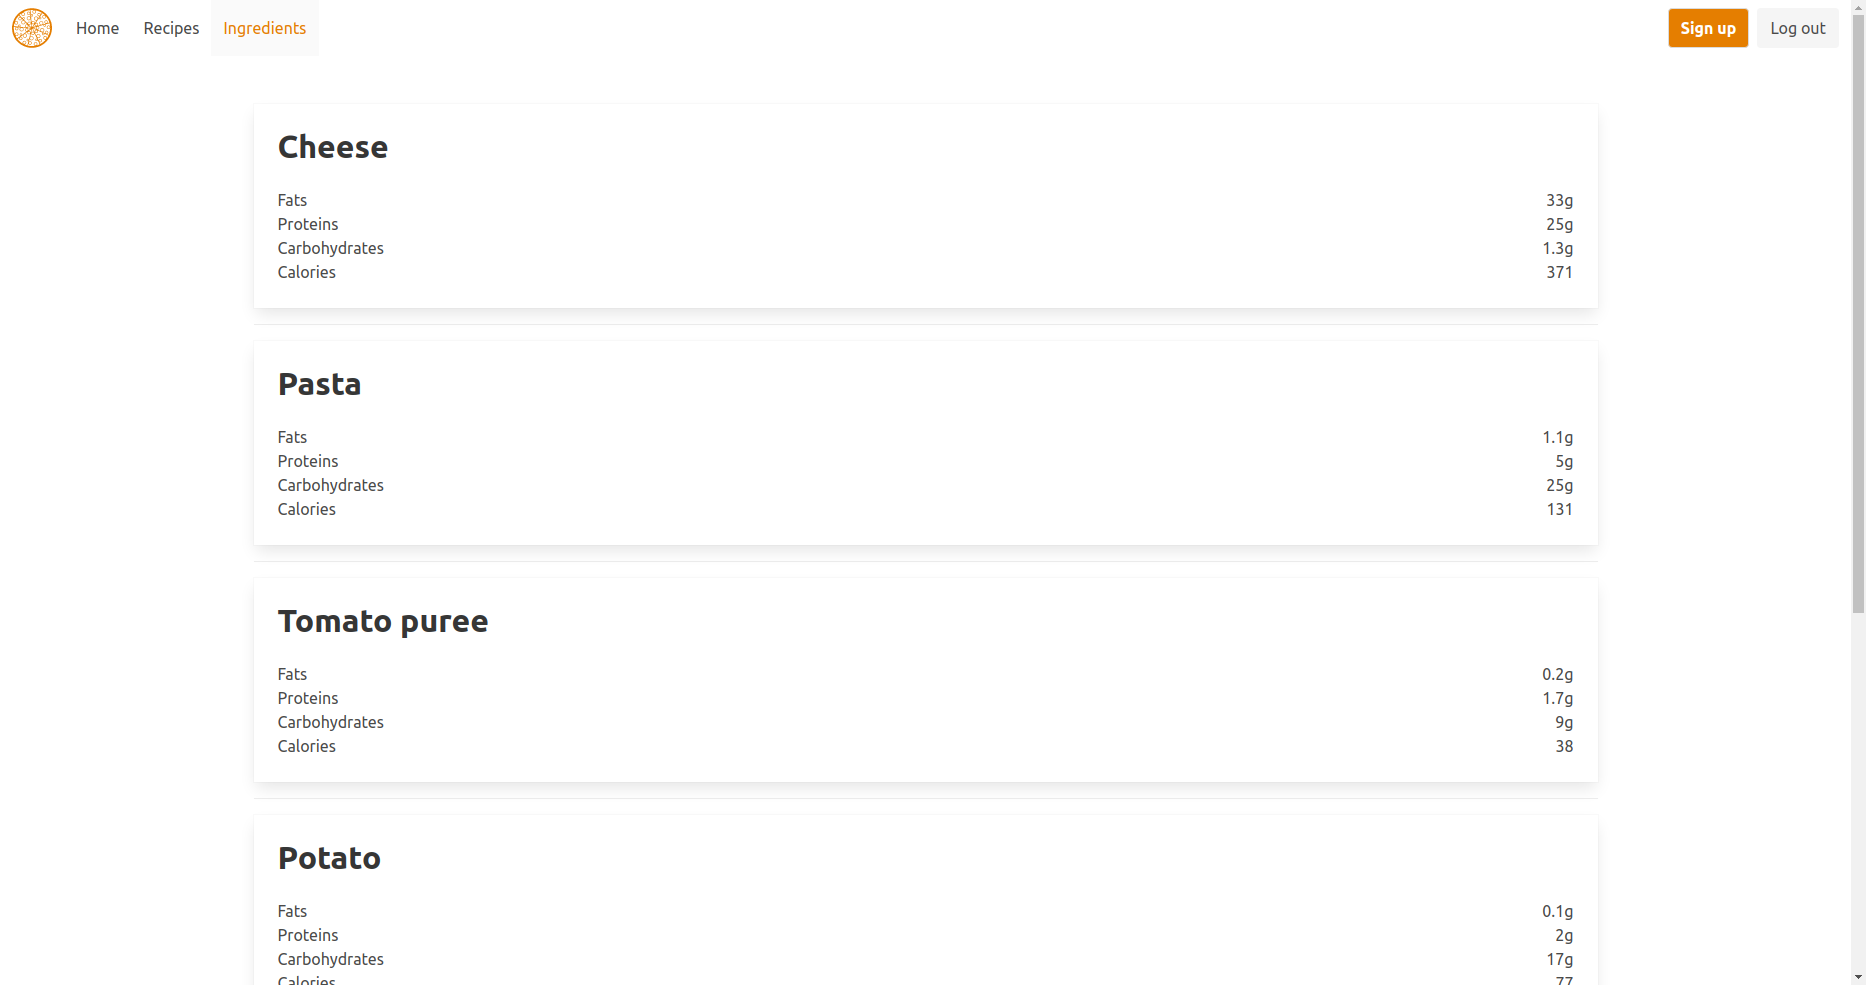
\includegraphics[width=15.5cm]{ingredients_list.png}
\newline
Każdy może wyświetlić wszystkie dostępne składniki i ich parametry
\subsection{Dodawanie przepisu}
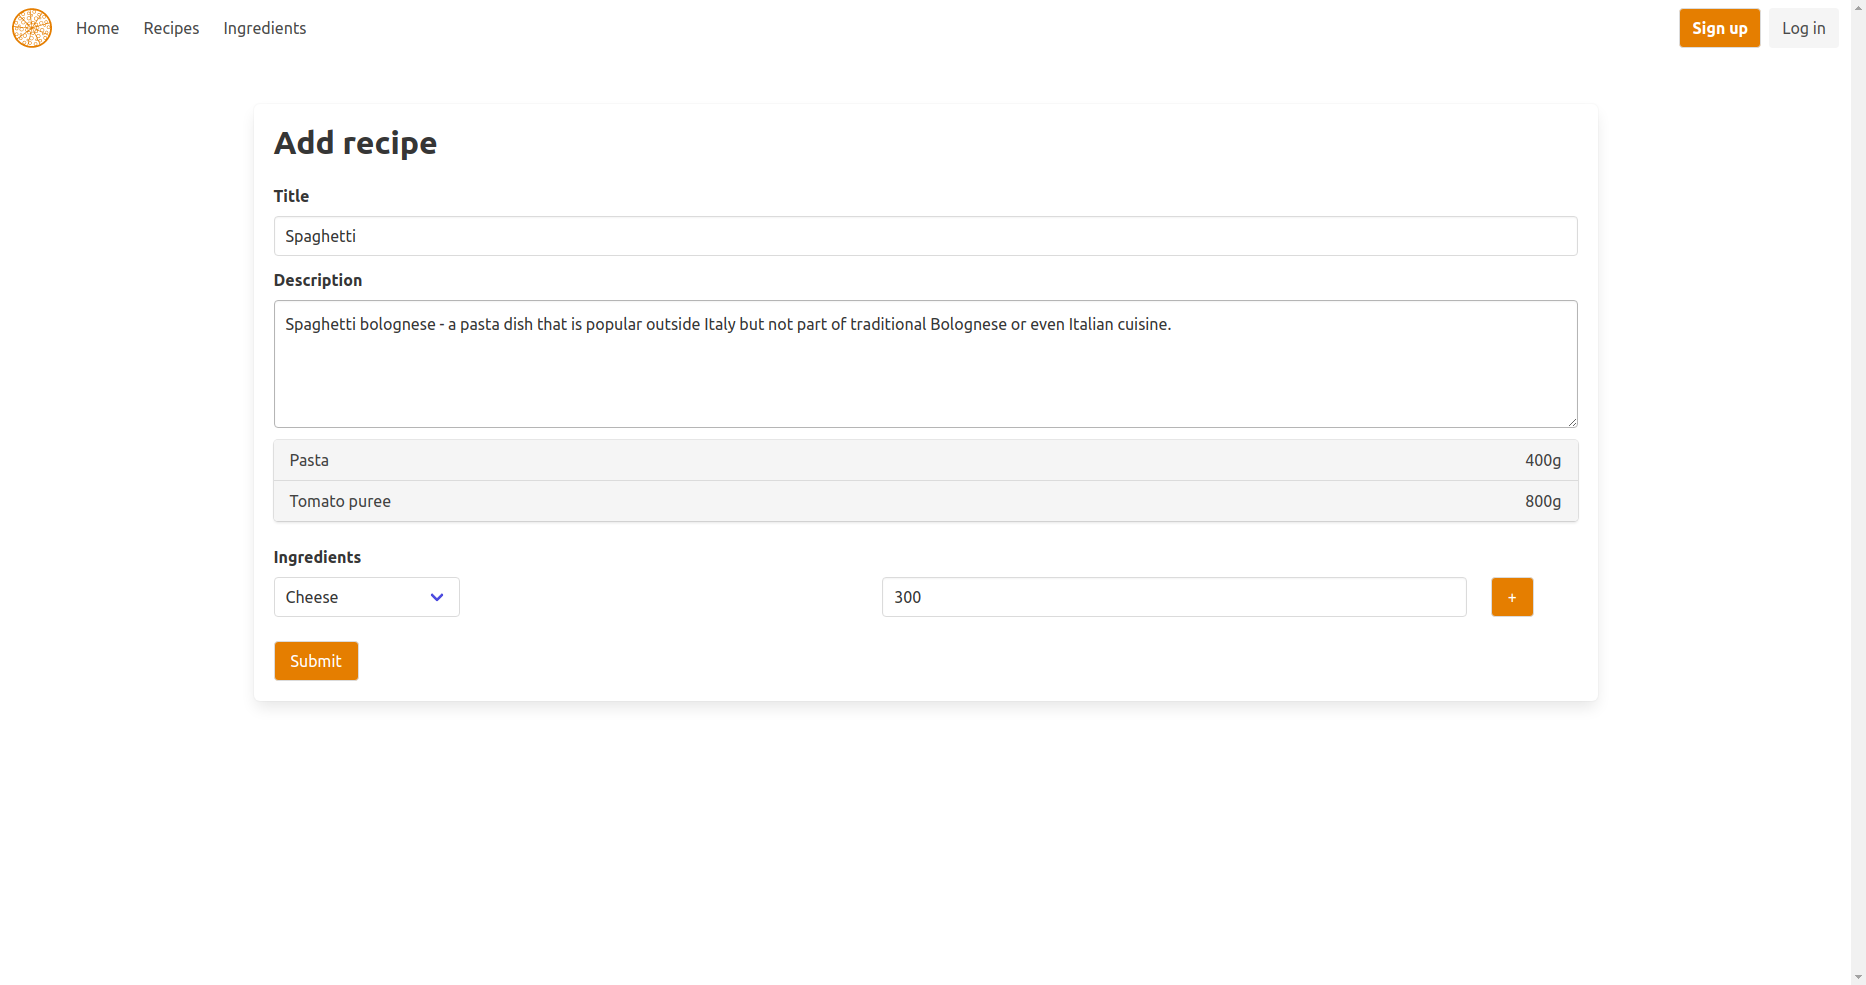
\includegraphics[width=15.5cm]{add_recipe.png}
\newline
Uwierzytelniony użytkownik może dodać przepis podając jego tytuł, opis oraz wybrane z listy składniki wraz z zadeklarowanymi ilościami
\subsection{Wyświetlanie listy przepisów}
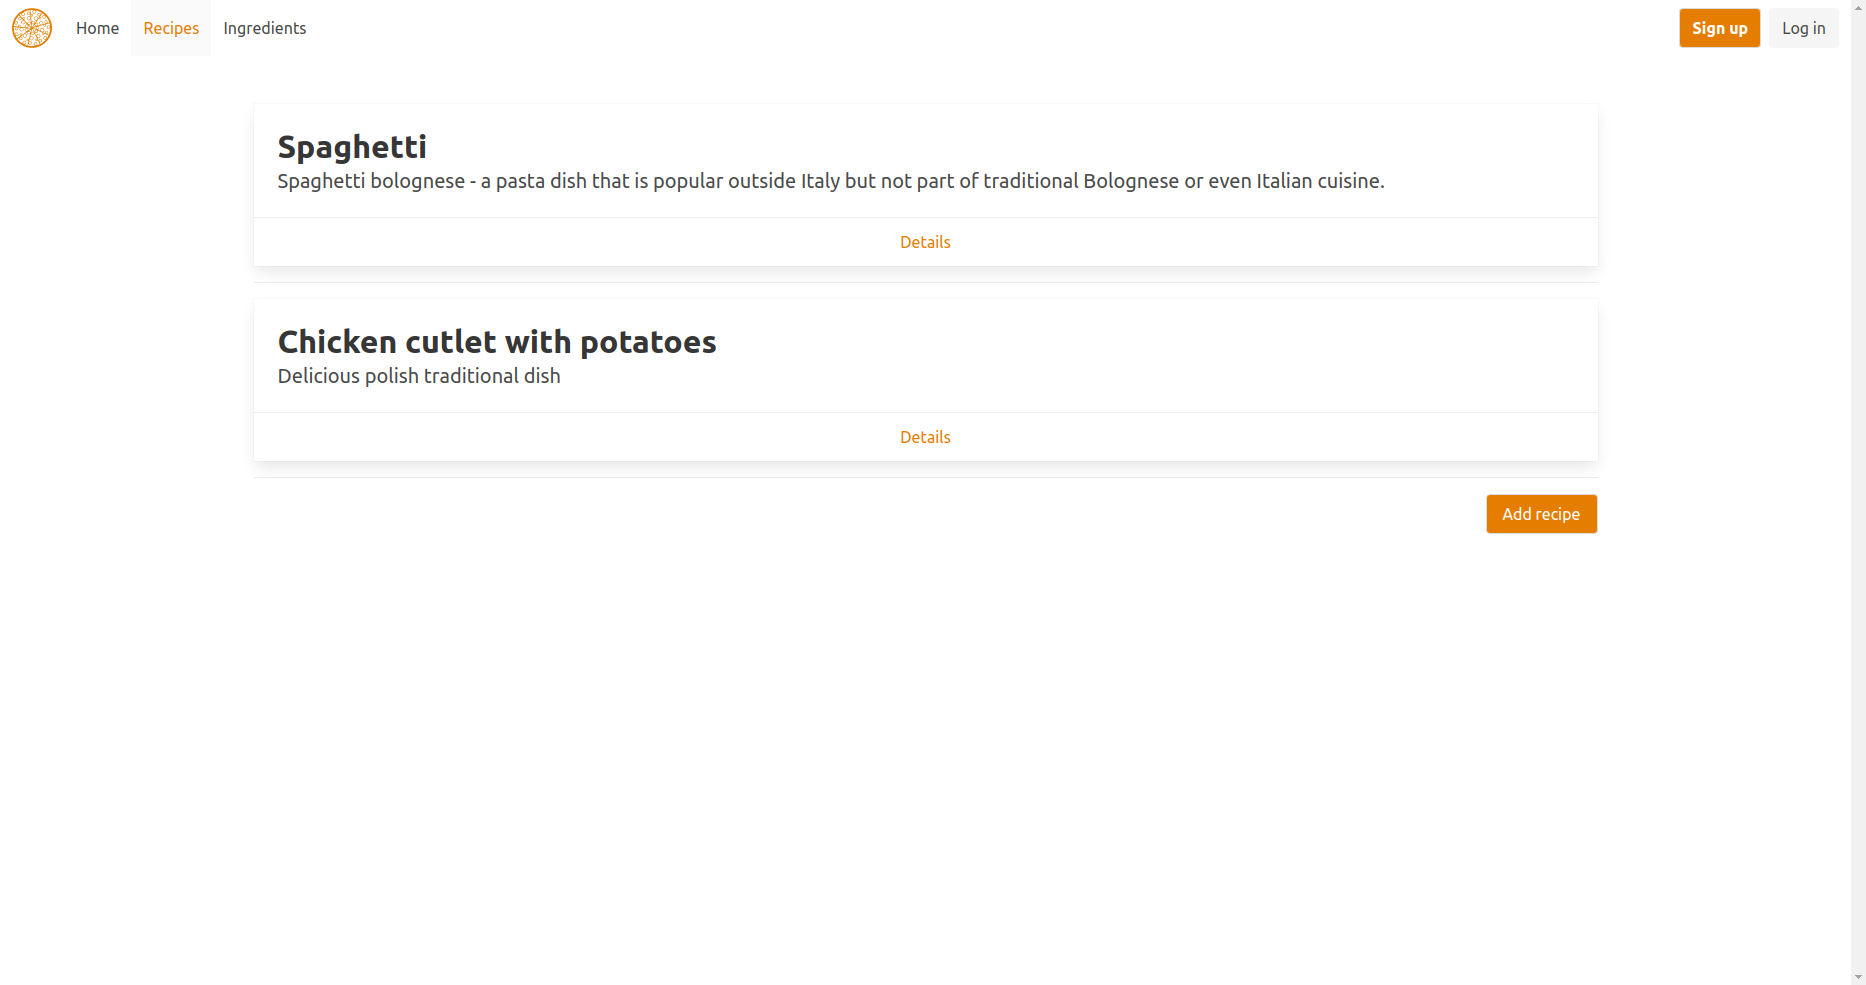
\includegraphics[width=15.5cm]{list_of_recipes.png}
\newline
Każdy może wyświetlić listę przepisów - ich tytuły i opisy
\subsection{Wyświetlanie szczegółów przepisu}
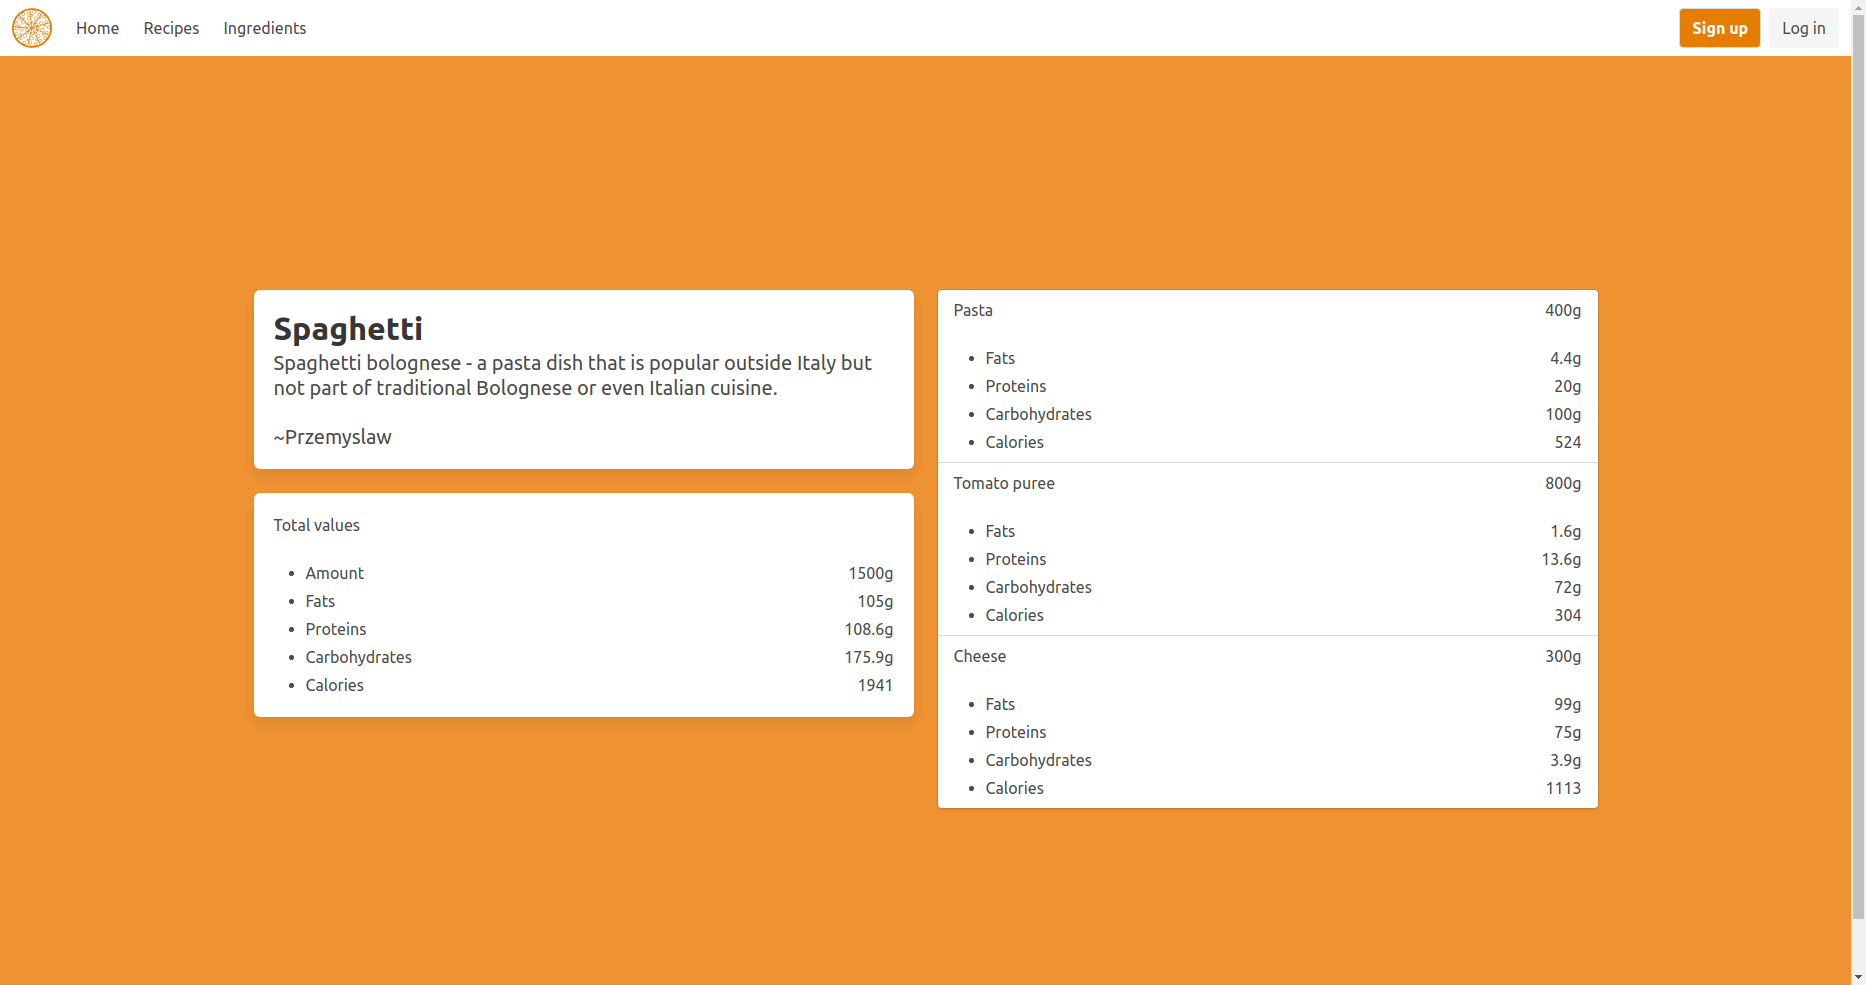
\includegraphics[width=15.5cm]{recipe_view.png}
\newline
Każdy może wyświetlić szczegóły przepisu - zawartość wartości odżywczych w danej ilości konkretnego składnika oraz w całym posiłku
\subsection{Wyświetlanie i dodawanie komentarzy do przepisu}
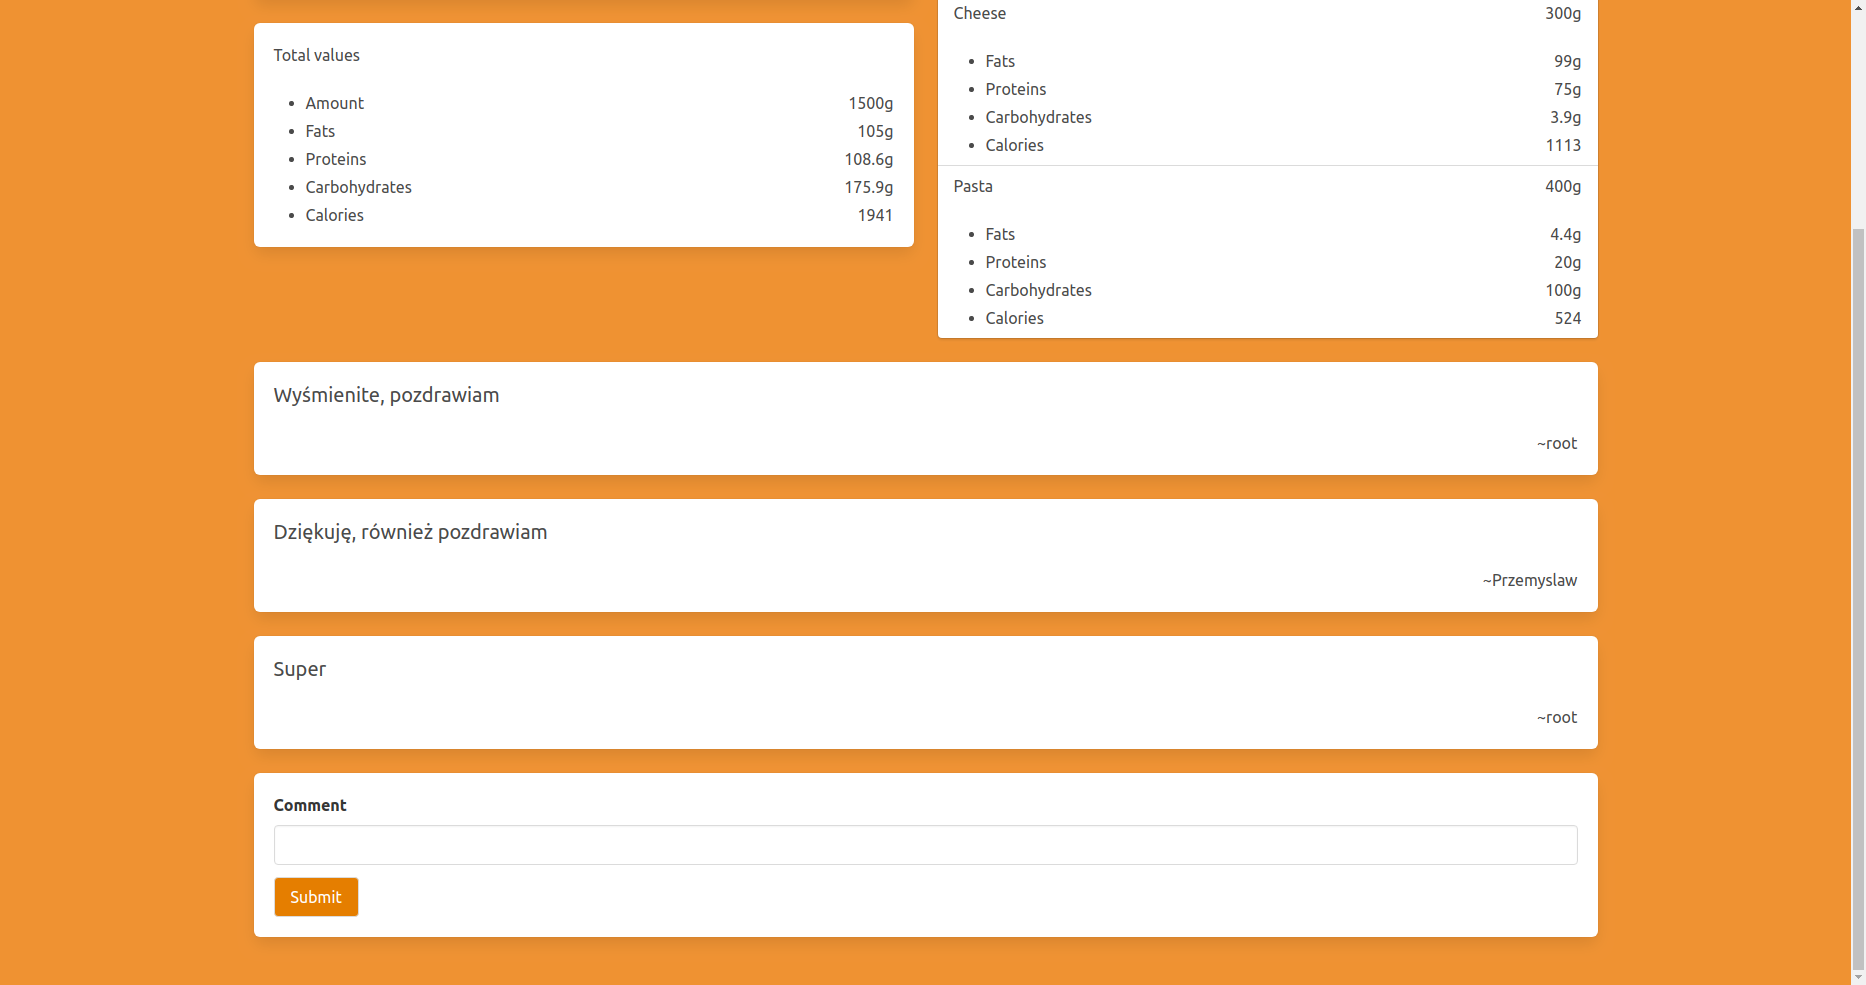
\includegraphics[width=15.5cm]{comments.png}
\newline
Komentarze mogą zostać wyświetlone przez każdego jednak tylko zalogowany użytkownik może dodać nowy komentarz

\section{Wnioski}
\begin{itemize}
    \item Dostępne obecnie narzędzia znacznie ułatwiają pracę z bazami danych, nie oznacza to jednak że można całkowicie obejść się bez znajomości relacyjnych baz danych. Pomimo interfejsu dostosowanego do języka programowania, którego używamy, nadal najistotniejszym elementem aplikacji bazodanowej jest przemyślana architektura bazy danych.
    \item Oddzielenie warstwy widoku zapewnia dużą swobodę implementacji oraz łatwiejszą skalowalność aplikacji internetowej.
    \item Aby przekształcić bazę danych w pełnoprawną i przydatną aplikację wystarczy rozszerzyć ją o kontrolę dostępu (system uprawnień) i przystępny protokół do komunikacji z użytkownikiem (w tym wypadku GUI)
\end{itemize}
\section{Możliwości rozwoju}
Jako, że aplikacja posiada rozdzielone bazę danych, serwer i aplikację po stronie klienta łatwo jest połączyć ją z innymi aplikacjami w podobnej tematyce oraz dodać nowe funkcje.
\begin{itemize}
    \item Wykorzystanie api w aplikacji pomagającej w trzymaniu diety, liczeniu kalorii
    \item Rozszerzenie funkcjonalności aplikacji o dopasowywanie przepisów do dietetycznych wymagań użytkownika
    \item Dodanie integracji z mediami społecznościowymi np.: udostępnianie przepisów
\end{itemize}
\end{document}